%%%%%%%% mlsys 2025 PROJECT REPORT FILE %%%%%%%%%%%%%%%%%

\documentclass{article}

% Recommended, but optional, packages for figures and better typesetting:
\usepackage{microtype}
\usepackage{graphicx}
\usepackage{subfigure}
\usepackage{booktabs} % for professional tables
\usepackage{natbib}
\usepackage{filecontents}
\usepackage{tikz}
\usetikzlibrary{arrows.meta, positioning, fit, calc}
\usepackage{hyperref}
\usepackage[utf8]{inputenc}




% Attempt to make hyperref and algorithmic work together better:
\newcommand{\theHalgorithm}{\arabic{algorithm}}

% Use the MLSys style template directly. The accepted option is used so the
% course project team members render in the PDF.
\usepackage[accepted]{mlsys2025}

\mlsystitlerunning{Paged-TierKV for High-Concurrency LLM Inference}

\begin{document}

\twocolumn[
\mlsystitle{Paged-TierKV: Compact Tiered KV Cache Management for High-Concurrency LLM Inference}

\begin{mlsysauthorlist}
\mlsysauthor{Martin Kang}{ini}
\mlsysauthor{Jingwu Wang}{scs}
\end{mlsysauthorlist}

\mlsysaffiliation{ini}{Information Networking Institute, Carnegie Mellon University, Pittsburgh, PA, USA}
\mlsysaffiliation{scs}{School of Computer Science, Carnegie Mellon University, Pittsburgh, PA, USA}

\mlsyscorrespondingauthor{Martin Kang}{lixuank@andrew.cmu.edu}
\mlsyscorrespondingauthor{Jingwu Wang}{jingwuwa@andrew.cmu.edu}

\mlsyskeywords{LLM inference, KV cache, memory systems, Triton, quantization}

\vskip 0.3in

\begin{abstract}
Long-context language-model serving is increasingly limited by the memory footprint and bandwidth cost of the key-value (KV) cache. We built Paged-TierKV, a block-level KV-cache manager that routes historical KV blocks into HOT full-precision storage, WARM int8 storage, or COLD metadata-only storage while preserving a paged logical view for attention. The system combines a C++ block manager, a Python policy/runtime layer, a compact state-separated tensor pool, and a decode-only Triton attention kernel. The central systems question is whether logical KV compression can become real physical memory savings without reintroducing full-cache reconstruction or destroying long-context quality. On TinyLlama with 1900-token prompts under high request concurrency, Paged-TierKV reduces the memory growth rate from roughly 43 MB/request for the dense baseline to roughly 27 MB/request near the boundary, and it succeeds at 512 concurrent requests where the dense baseline runs out of memory. The system does not outperform the dense baseline in raw throughput; instead, its strongest result is converting logical KV compression into physical memory savings while maintaining usable quality and throughput under high KV pressure.
\end{abstract}
]

\printAffiliationsAndNotice{}

\section{Introduction}

Autoregressive large language model (LLM) inference stores a key and value tensor for every generated or prefetched token in every decoder layer. This KV cache avoids recomputing past activations, but its footprint grows linearly with context length, number of layers, number of KV heads, head dimension, and number of active requests. More concretely, the dense fp16 KV footprint is proportional to
$
2 \cdot R \cdot L \cdot T \cdot H_{kv} \cdot D \cdot 2
$
bytes, where $R$ is the number of resident requests, $L$ is the layer count, $T$ is context length, $H_{kv}$ is the number of KV heads, and $D$ is head dimension. Model weights are fixed after loading, but this cache grows with workload pressure. In long-context or high-concurrency serving, the KV cache can therefore become the dominant incremental working set.

Paged-TierKV targets this systems bottleneck. The project asks whether a paged, block-level cache can preserve the important parts of history in high precision, compress less important history, and expose real memory savings without reconstructing the full KV cache on every decode step. This distinction between logical and physical savings is important. A policy may mark most blocks as compressed, but if the implementation still allocates dense HOT and WARM capacity for every physical block, peak GPU memory will not improve. Earlier versions of the system demonstrated the logical idea but were limited by Python-side reconstruction and dense pool allocation. The final system uses a compact state-separated pool and Triton decode path so that HOT blocks consume fp16 storage, WARM blocks consume int8 storage plus metadata, and COLD blocks consume no dense KV storage.

Our main contribution is an end-to-end prototype integrated into a Hugging Face LLaMA-style model path. It implements block allocation, attention-based policy enforcement, compact state migration, decode-time fused dequantization/attention, and memory-realism telemetry. The evaluation shows a memory-scaling advantage under high KV pressure: in the main TinyLlama experiment, the dense baseline succeeds up to 448 concurrent 1900-token requests and fails at 512, while Paged-TierKV succeeds at 512. The result is not a universal throughput win. TierKV pays overhead for WARM dequantization, metadata indirection, and request-local decode scheduling. Its strongest validated claim is that compact tiered KV storage lowers the memory growth slope and extends the supported load before out-of-memory. We also run a 7B MHA-style Vicuna extension, which strengthens the memory-scaling story but does not produce a throughput crossover.

\section{Problem}

The dense KV-cache baseline stores every historical token in fp16 until the request ends. This is simple and fast: attention reads a contiguous representation with no per-block state checks, no dequantization, and no policy bookkeeping. The drawback is that memory grows with total active context. If the serving system holds many concurrent long-context requests, dense KV quickly pushes the GPU toward its memory boundary even if the model weights themselves fit comfortably.

Two straightforward alternatives are insufficient on their own. Uniform quantization can reduce cache bytes, but it applies the same approximation to recent and important history and can introduce dequantization overhead on every attention read. Pure sparsification or token dropping saves more memory, but it can destroy retrieval or QA behavior when the removed blocks contain the answer. Our Qasper results demonstrate both sides: pure quantization preserves most quality but is slow, while pure sparsification has high compression and higher throughput but collapses F1.

Paged-TierKV addresses the following systems question: can we combine paged metadata, mixed precision, and selective eviction so that the cache uses less physical memory while preserving enough context for long-context QA? The central tradeoff is three-way. HOT fp16 blocks maximize fidelity and simple reads but consume dense memory. WARM int8 blocks retain information at lower memory cost but require dequantization during attention. COLD blocks remove resident KV storage entirely but lose the represented content. A useful system must therefore track block state cheaply, migrate blocks safely, avoid full-cache reconstruction in the decode hot path, and expose truthful memory metrics. The project is successful only if compression affects actual allocated GPU memory, not just a logical accounting table.
\section{Related Work}

Paged KV-cache serving systems such as paged attention \citep{kwon2023efficient} decouple logical sequence layout from physical GPU memory allocation. They motivate this project because they show that block tables are a practical interface between model-level attention and allocator-level memory management. Paged-TierKV uses the same broad idea of a logical block table, but adds state-dependent storage tiers and compression rather than only paging dense KV blocks.

KV-cache quantization reduces the byte footprint of historical keys and values \citep{liu2023kivi, pmlr-v202-sheng23a}. Our WARM tier follows this direction, using int8 storage with scale and zero-point metadata. The project differs from uniform quantization by reserving a small set of HOT blocks in fp16, selected by attention-derived policy, so important recent or high-attention blocks need not pay quantization error.

KV sparsification and token eviction reduce memory by dropping parts of the context \citep{zhang2023h2o, xiao2023efficient}. Our COLD tier is a controlled version of this idea. The evaluation confirms the risk: pure sparsification achieves low resident KV but Qasper F1 collapses, while HOT+WARM keeps F1 close to the dense baseline.

Long-context benchmarks and LLM serving frameworks provide the workload context for this project. We use a Qasper subset from LongBench \citep{bai-etal-2024-longbench} for quality and staged synthetic concurrency to drive KV pressure, testing on models such as TinyLlama \citep{zhang2024tinyllama} and Vicuna \citep{vicuna2023}. The implementation relies on PyTorch \citep{paszke2019pytorch}, Hugging Face Transformers \citep{wolf2020transformers}, Triton \citep{tillet2019triton}, and Modal \citep{modal2024} for GPU execution.

\section{Overview}

Paged-TierKV treats each layer's KV history as a sequence of fixed-size blocks. Each logical block is assigned one of three states. HOT blocks are stored in fp16 and are used for attention without quantization. WARM blocks are stored in uint8 with per-token metadata and dequantized inside the decode attention kernel. COLD blocks keep metadata and valid length but no resident dense KV storage.

\begin{figure}[t]
\begin{center}
\resizebox{\linewidth}{!}{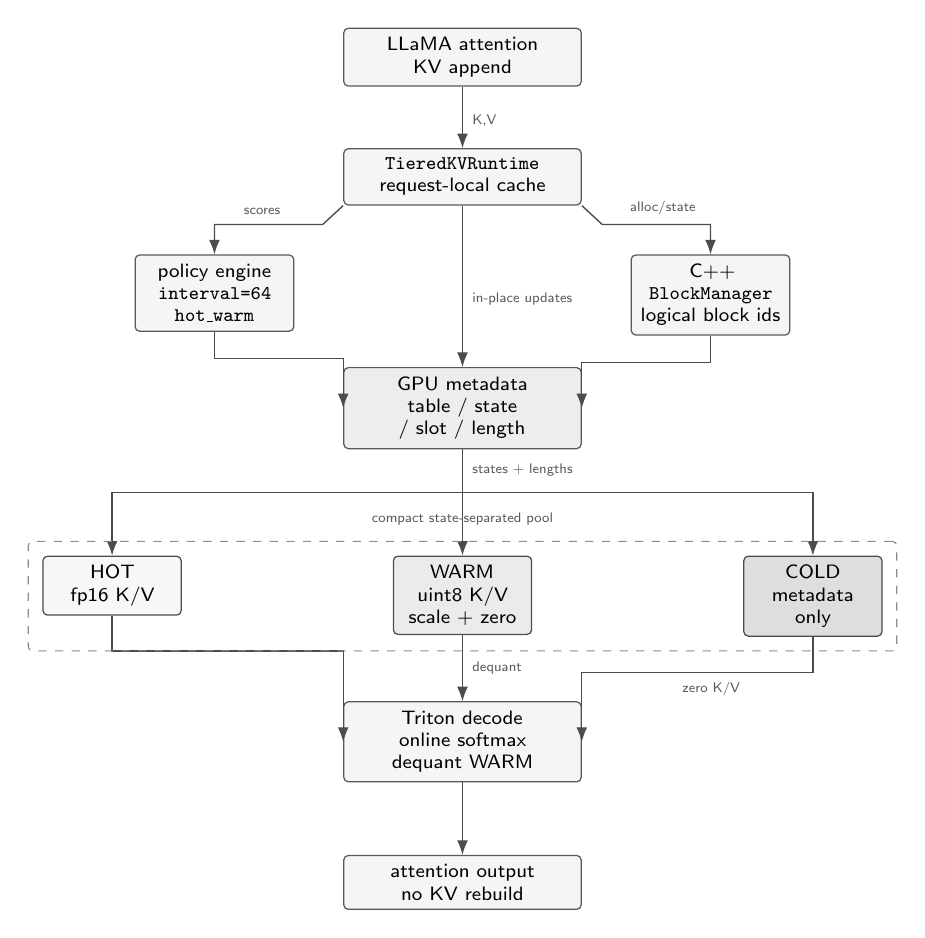
\begin{tikzpicture}[
  font=\scriptsize\sffamily,
  >=Latex,
  node distance=0.72cm and 0.62cm,
  box/.style={
    draw=black!65,
    rounded corners=1.6pt,
    align=center,
    minimum height=0.66cm,
    text width=2.78cm,
    fill=black!4,
    line width=0.45pt
  },
  side/.style={
    draw=black!65,
    rounded corners=1.6pt,
    align=center,
    minimum height=0.58cm,
    text width=1.78cm,
    fill=black!4,
    line width=0.45pt
  },
  meta/.style={
    draw=black!65,
    rounded corners=1.6pt,
    align=center,
    minimum height=0.66cm,
    text width=2.78cm,
    fill=black!7,
    line width=0.45pt
  },
  pool/.style={
    draw=black!70,
    rounded corners=1.6pt,
    align=center,
    minimum height=0.60cm,
    text width=1.52cm,
    line width=0.45pt
  },
  arrow/.style={->, line width=0.5pt, draw=black!70},
  note/.style={font=\tiny\sffamily, text=black!65}
]

% 中轴主流程：全部严格共线
\node[box] (attn) {LLaMA attention\\KV append};
\node[box, below=0.78cm of attn] (runtime) {\texttt{TieredKVRuntime}\\request-local cache};
\node[meta, below=2.05cm of runtime] (metadata) {GPU metadata\\table / state / slot / length};
\node[box, below=3.20cm of metadata] (triton) {Triton decode\\online softmax\\dequant WARM};
\node[box, below=0.92cm of triton] (out) {attention output\\no KV rebuild};

% 左右辅助模块：围绕 runtime 对称
\node[side, below left=0.62cm and 0.62cm of runtime] (policy) {policy engine\\\texttt{interval=64}\\\texttt{hot\_warm}};
\node[side, below right=0.62cm and 0.62cm of runtime] (manager) {C++ \texttt{BlockManager}\\logical block ids};

% 三层池：同一水平线
\node[pool, fill=black!3, below left=1.35cm and 2.05cm of metadata] (hot) {HOT\\fp16 K/V};
\node[pool, fill=black!8, below=1.35cm of metadata] (warm) {WARM\\uint8 K/V\\scale + zero};
\node[pool, fill=black!13, below right=1.35cm and 2.05cm of metadata] (cold) {COLD\\metadata only};

% 上半部分连线
\draw[arrow] (attn) -- node[right, note, pos=0.55]{K,V} (runtime);
\draw[arrow] (runtime.south west) -- ++(-0.26,-0.24) -| node[pos=0.28, above, note]{scores} (policy.north);
\draw[arrow] (runtime.south east) -- ++(0.26,-0.24) -| node[pos=0.28, above, note]{alloc/state} (manager.north);
\draw[arrow] (policy.south) -- ++(0,-0.34) -| (metadata.west);
\draw[arrow] (manager.south) -- ++(0,-0.34) -| (metadata.east);
\draw[arrow] (runtime.south) -- node[right, note, pos=0.58]{in-place updates} (metadata.north);

% metadata 到三层池：左右对称、同层展开
\draw[arrow] (metadata.south) -- ++(0,-0.55) -| (hot.north);
\draw[arrow] (metadata.south) -- node[right, note, pos=0.2]{states + lengths} (warm.north);
\draw[arrow] (metadata.south) -- ++(0,-0.55) -| (cold.north);

% 三层池到 Triton
\draw[arrow] (hot.south) -- ++(0,-0.45) -| (triton.west);
\draw[arrow] (warm.south) -- node[right, note, pos=0.5]{dequant} (triton.north);
\draw[arrow] (cold.south) -- ++(0,-0.45) -| node[pos=0.22, below, note]{zero K/V} (triton.east);

\draw[arrow] (triton) -- (out);

% 三层池包围框
\node[
  draw=black!45,
  rounded corners=1.6pt,
  dashed,
  fit=(hot)(warm)(cold),
  inner sep=0.18cm,
  label={[note, yshift=0.08cm]above:compact state-separated pool}
] {};

\end{tikzpicture}}
\end{center}
\caption{Paged-TierKV system overview.}
\label{fig:overview}
\end{figure}

The default configuration used in the final results is \texttt{policy\_interval=64}, \texttt{policy\_on\_new\_block=False}, and \texttt{policy\_mode=hot\_warm}. Prefill remains eager and computes a policy signal once for the prompt. Decode uses a Triton kernel for query length one. The final evaluation separates the main TinyLlama high-concurrency result from a supporting 7B Vicuna experiment, because the extension tests a different question: whether a larger MHA model creates enough KV pressure for a throughput crossover.

\section{System Design}

\subsection{Block Metadata and Runtime}

The C++ \texttt{BlockManager} is the metadata source for block allocation and state transitions. It gives each logical KV block a stable identity and tracks whether that block is HOT, WARM, or COLD. The Python \texttt{TieredKVRuntime} owns the model-facing cache object, policy engine, tensor pool, layer state, profiling counters, and memory telemetry. This split keeps the allocator/policy interface explicit while allowing the Hugging Face model path to treat TierKV as a cache implementation.

Each layer has a logical table of active blocks, block states, slot indices, and block lengths. The block table preserves logical order. The state table selects the HOT, WARM, or COLD read path. The slot-index table maps a logical block to its current state-specific storage slot. The length table masks unused positions in the final partial block. This metadata stays resident on GPU for the decode path. The attention layer prefers the runtime attached to \texttt{past\_key\_values}, which allows multiple active TierKV caches to coexist. In the staged benchmark, concurrency is implemented as many independent batch-1 requests rather than true batched attention; this preserves the current Triton contract while creating real aggregate KV pressure.

\subsection{Compact State-Separated Pool}

The final memory result depends on separating logical block identity from physical storage slots. A dense tiered pool can report many WARM or COLD blocks but still allocate enough tensor capacity for every block to be HOT or WARM. That design shows logical compression but not physical savings. Paged-TierKV's compact pool instead allocates independent HOT and WARM storage. HOT slots store fp16 keys and values. WARM slots store uint8 keys and values plus fp16 scale/zero metadata. COLD blocks store no dense KV tensor.

State transitions migrate slots explicitly. A new decode block allocates a HOT slot. HOT-to-WARM migration quantizes from the HOT slot into a WARM slot and frees the HOT slot. WARM-to-HOT migration, when used by the policy, allocates a HOT slot, dequantizes, and frees the WARM slot. HOT/WARM-to-COLD frees any dense slot and keeps only metadata. COLD promotion is not supported in the current policy, matching the irreversible COLD semantics used in the implementation. This state-separated layout is the key change that converts the policy's logical compression into reduced physical KV allocation.

\subsection{Policy Scheduling}

The policy protects sink/recent blocks and selects additional HOT blocks from attention-derived block scores. The default HOT+WARM mode keeps selected blocks HOT and demotes all other live blocks to WARM. HOT+WARM+COLD additionally uses a WARM budget and demotes remaining blocks to COLD, which improves compression but hurts quality. The policy is deliberately not run on every new block in the final configuration; \texttt{policy\_on\_new\_block=False} lets \texttt{policy\_interval} control the update cadence. Prior profiling showed policy-path work, not the Triton decode kernel alone, was a main bottleneck. The final \texttt{policy\_interval=64} setting therefore amortizes scoring and migration while keeping the block state stable enough to preserve Qasper quality.

\subsection{Triton Decode Path}

For decode, where query length is one, the model calls \texttt{tierkv\_decode\_attention}. The kernel launches over query heads, maps each query head to a KV head, iterates over logical blocks, and reads the state and slot index for each block. HOT loads fp16 K/V directly. WARM loads uint8 K/V and dequantizes inside the kernel. COLD contributes zero K/V while preserving the valid sequence positions in the softmax denominator. This avoids Python-side \texttt{torch.cat} reconstruction in the decode hot path, so sequence-length-dependent work is pushed into the GPU kernel rather than repeated Python tensor construction. The implementation remains decode-only and batch-1 per request; the multi-request benchmark scales pressure by keeping many independent caches resident.

\subsection{Telemetry}

The runtime reports active HOT/WARM/COLD block counts, logical resident KV, dense-equivalent KV, physical KV allocation, compression ratios, and pool utilization. Dense-equivalent KV estimates how much fp16 KV the active blocks would consume with no compression. Logical resident KV counts the represented state: fp16 bytes for HOT, int8 bytes plus metadata for WARM, and zero dense bytes for COLD. Physical KV allocation counts actual allocated HOT/WARM pools using tensor sizes. Peak memory is measured with \texttt{torch.cuda.max\_memory\_allocated()} in clean runs. These counters are important because early dense-pool versions showed logical compression without corresponding physical savings. The final tables report both logical and physical compression to distinguish policy effectiveness from allocator effectiveness.

\section{Evaluation}

\subsection{Setup}

All final experiments run on Modal with an NVIDIA A10G. The main model is TinyLlama-1.1B-Chat with legal 1900-token inputs, leaving room under the 2048-token context limit for generation. Quality uses 50 Qasper examples from LongBench, left-truncated to 1900 input tokens and decoded for short answers. Throughput scaling uses decode-only timing after prefill, so the high-concurrency curves measure the incremental decode regime where KV pressure matters most. The high-pressure benchmark holds multiple independent batch-1 requests resident and decodes them round-robin.

We compare a dense Hugging Face baseline, pure quantization, pure sparsification, and Paged-TierKV. The primary Paged-TierKV configuration is HOT+WARM with hot budget 8. Memory tables use peak allocated memory, not reserved memory, and report TierKV's logical and physical KV counters before cache cleanup. The supporting extension uses \texttt{lmsys/vicuna-7b-v1.5}, a LLaMA-compatible MHA model with hidden size 4096, 32 layers, 32 attention heads, 32 KV heads, and max position embeddings 4096.

\subsection{Quality and Compression}

Table~\ref{tab:qasper} shows that HOT+WARM Paged-TierKV preserves most of the baseline Qasper F1, while pure sparsification collapses. The budget-8 configuration reaches 10.67 F1 versus 11.17 for the dense baseline, a small absolute loss relative to the failure mode of pure sparsification at 0.93 F1. This is the quality argument for keeping most non-HOT blocks WARM rather than COLD. Its physical compression is 1.68$\times$ on the Qasper run, showing that the compact pool turns WARM placement into actual lower KV allocation rather than only a logical label.

\begin{table}[t]
\caption{Qasper-50 quality and memory summary at 1900 input tokens.}
\label{tab:qasper}
\vskip 0.15in
\begin{center}
\begin{small}
\begin{tabular}{lrrrr}
\toprule
Configuration & Peak MB & F1 & tok/s & \begin{tabular}{@{}r@{}}Phys. \\ comp.\end{tabular} \\
\midrule
Baseline & 2238.56 & 11.17 & 53.29 & -- \\
\begin{tabular}{@{}l@{}}Pure Quantization\end{tabular} & 2220.81 & 10.75 & 16.27 & 1.75$\times$ \\
\begin{tabular}{@{}l@{}}Pure Sparsification\end{tabular} & 2198.53 & 0.93 & 32.94 & 29.99$\times$ \\
\begin{tabular}{@{}l@{}}Paged-TierKV, \\ budget 4\end{tabular} & 2220.46 & 10.55 & 16.44 & 1.77$\times$ \\
\begin{tabular}{@{}l@{}}Paged-TierKV, \\ budget 8\end{tabular} & 2222.87 & 10.67 & 16.75 & 1.68$\times$ \\
\bottomrule
\end{tabular}
\end{small}
\end{center}
\vskip -0.1in
\end{table}

The tier-mode ablation in Table~\ref{tab:tiermodes} clarifies the quality-memory tradeoff. HOT-only preserves baseline quality but offers no compression: its physical compression is 0.99$\times$, effectively dense storage. HOT+WARM keeps quality close to baseline and gives meaningful physical compression. HOT+WARM+COLD improves physical compression to 4.40$\times$ but reduces Qasper F1 to 1.47, so it is not the quality-preserving default. This result is useful because it separates two claims. TierKV can aggressively reduce memory with COLD blocks, but the practical default must keep enough WARM information to answer long-context questions.

\begin{table}[t]
\caption{Tier-mode ablation. HOT+WARM is the final default because it preserves quality while compressing physical KV.}
\label{tab:tiermodes}
\vskip 0.15in
\begin{center}
\begin{small}
\begin{tabular}{lrrrr}
\toprule
Mode & F1 & tok/s & HOT/WARM/COLD & \begin{tabular}{@{}r@{}}Phys. \\ comp.\end{tabular} \\
\midrule
HOT-only & 11.16 & 23.53 & 2662/0/0 & 0.99$\times$ \\
HOT+WARM & 10.67 & 12.77 & 220/2442/0 & 1.68$\times$ \\
HOT+WARM+COLD & 1.47 & 19.80 & 220/704/1738 & 4.40$\times$ \\
\bottomrule
\end{tabular}
\end{small}
\end{center}
\vskip -0.1in
\end{table}

The distinction between logical and physical compression matters throughout the evaluation. Pure sparsification reports very high compression because almost all non-protected blocks become COLD, but the quality loss makes that point unusable. HOT+WARM has a lower compression factor, around 1.68$\times$ physical compression on Qasper, but it preserves the semantic information needed by the QA task. This is the operating point used for the high-pressure scaling results.

\subsection{High-Concurrency Scaling}

The main systems result is the staged TinyLlama concurrency benchmark. Table~\ref{tab:scaling} compresses the curve to representative points. TierKV's peak memory grows more slowly than the dense baseline. The memory gap grows from 529.50 MB at 32 requests to 7239.73 MB at 448 requests. In the boundary run, the dense baseline succeeds at 448 requests but fails at 512 with CUDA out of memory. Paged-TierKV succeeds at 512 requests with 15159.07 MB peak memory, 12952.00 MB physical KV allocation, and 1.65$\times$ physical KV compression.

\begin{table*}[t]
\caption{Representative TinyLlama high-concurrency scaling points with 1900-token prompts. Throughput ratio is TierKV divided by dense baseline.}
\label{tab:scaling}
\vskip 0.15in
\begin{center}
\begin{small}
\begin{tabular}{rrrrrrr}
\toprule
Requests & Baseline MB & TierKV MB & TierKV phys. KV MB & Dense-eq. KV MB & Throughput ratio & Status \\
\midrule
32 & 3439.77 & 2910.27 & 792.00 & 1317.94 & 0.88$\times$ & both OK \\
160 & 8823.58 & 6180.70 & 4037.00 & 6699.69 & 0.80$\times$ & both OK \\
320 & 15536.85 & 10267.70 & 8081.00 & 13410.38 & 0.68$\times$ & both OK \\
448 & 20711.66 & 13471.93 & 11256.00 & 18583.12 & 0.88$\times$ & both OK \\
512 & OOM & 15159.07 & 12952.00 & 21373.00 & -- & baseline OOM \\
\bottomrule
\end{tabular}
\end{small}
\end{center}
\vskip -0.1in
\end{table*}

Table~\ref{tab:slopes} summarizes the memory slopes printed by the staged runner. The dense baseline grows at roughly 42--43 MB/request across TinyLlama stages. TierKV grows at roughly 25--27 MB/request. This is the clearest evidence that the compact pool changes the scaling curve, not just one high-load point. The 7B extension shows the same pattern at a larger per-request scale: baseline memory grows faster than TierKV at both 1024-token and 1536-token contexts.

\begin{table}[t]
\caption{Peak-memory slope summary. Lower MB/request means better memory scaling as concurrency grows.}
\label{tab:slopes}
\vskip 0.15in
\begin{center}
\begin{small}
\begin{tabular}{lrr}
\toprule
Range & Baseline & TierKV \\
\midrule
TinyLlama 32--160 & 42.06 & 25.55 \\
TinyLlama 192--320 & 43.01 & 26.08 \\
TinyLlama 384--448 & 43.26 & 26.90 \\
Vicuna 1024, 1--12 & 536.00 & 339.63 \\
Vicuna 1536, 1--8 & 791.65 & 479.32 \\
\bottomrule
\end{tabular}
\end{small}
\end{center}
\vskip -0.1in
\end{table}

\begin{figure}[t]
\begin{center}
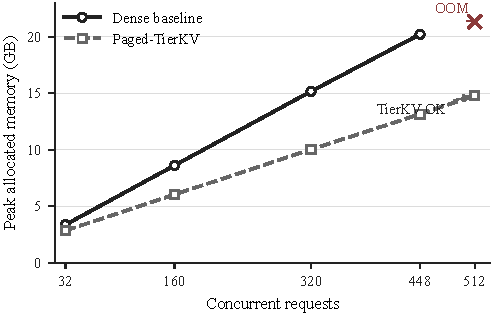
\includegraphics[width=\linewidth]{fig_memory_scaling.pdf}
\end{center}
\caption{Peak memory scaling for the TinyLlama high-concurrency benchmark.}
\label{fig:memory-scaling}
\end{figure}

\begin{figure}[t]
\begin{center}
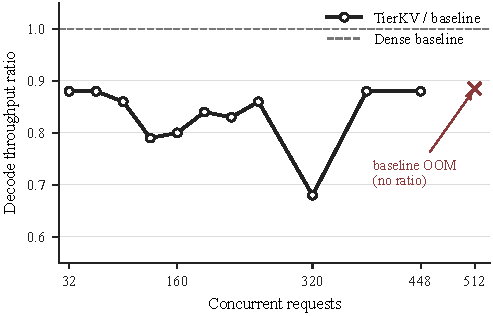
\includegraphics[width=\linewidth]{fig_throughput_ratio.pdf}
\end{center}
\caption{Throughput ratio for the TinyLlama high-concurrency benchmark.}
\label{fig:throughput-ratio}
\end{figure}

The boundary summary is shown in Table~\ref{tab:boundary}. This is the strongest result in the project: the compact state-separated pool converts logical compression into physical memory savings large enough to extend the maximum supported concurrent load. It also clarifies the role of throughput. TierKV is not faster than dense baseline at matched successful points, but the baseline cannot produce a 512-request throughput number because it fails before the measurement completes.

\begin{table}[t]
\caption{Failure boundary in the final TinyLlama staged sweep.}
\label{tab:boundary}
\vskip 0.15in
\begin{center}
\begin{small}
\begin{tabular}{lrrr}
\toprule
Method & Max OK req. & Total ctx. tokens & Failure \\
\midrule
Baseline & 448 & 851200 & OOM at 512 \\
Paged-TierKV & 512 & 972800 & none observed \\
\bottomrule
\end{tabular}
\end{small}
\end{center}
\vskip -0.1in
\end{table}

\subsection{7B Extension}

The 7B extension tests whether a larger MHA-style model becomes KV-bound enough for TierKV to exceed dense throughput. It does not. However, the extension supports the memory-scaling story on a model with much larger per-request KV footprint. The passkey sanity check confirms both baseline and TierKV preserve the expected passkey. At 1024-token context, the TierKV/dense throughput ratio improves from 0.44$\times$ to 0.77$\times$ as requests increase from 1 to 12, while the memory gap grows from 169.65 MB to 2329.80 MB. At 1536-token context, the ratio improves from 0.45$\times$ to 0.75$\times$, while the memory gap grows from 301.42 MB to 2487.73 MB.

\begin{table}[t]
\caption{Vicuna-7B MHA extension summary. No throughput crossover is observed.}
\label{tab:extension}
\vskip 0.15in
\begin{center}
\begin{small}
\begin{tabular}{lrrrr}
\toprule
Context & \begin{tabular}{@{}r@{}}Req. \\ range\end{tabular} & Ratio trend & Gap trend MB & \begin{tabular}{@{}r@{}}Last \\ comp.\end{tabular} \\
\midrule
1024 & 1--12 & 0.44--0.77$\times$ & 169.65--2329.80 & 1.60$\times$ \\
1536 & 1--8 & 0.45--0.75$\times$ & 301.42--2487.73 & 1.70$\times$ \\
\bottomrule
\end{tabular}
\end{small}
\end{center}
\vskip -0.1in
\end{table}

This extension should be read as supporting evidence rather than the main result. It uses a different model and lower request counts because a 7B model has much higher base memory. The useful observation is that the same slope pattern appears: TierKV memory grows more slowly as concurrency increases. The throughput gap narrows with pressure, but it does not close. That means the current implementation's extra WARM-path and metadata overhead still dominates before a raw throughput crossover appears.

\subsection{Discussion}

Paged-TierKV does not make decode universally faster than the dense baseline. The Triton path avoids full-cache reconstruction, but WARM dequantization, metadata indirection, policy bookkeeping, and per-request serving overhead still cost throughput. The current benchmark also uses many independent batch-1 requests rather than a fused batched serving kernel, so it does not exploit batching to amortize launch and metadata overhead. The system result is therefore not a raw speedup claim. It is a memory-scaling claim: for high KV pressure, the compact pool lowers the physical memory slope and allows a larger successful load.

The results also show why memory-realism telemetry was necessary. Logical resident KV measures what the policy intends to keep, while physical KV allocation measures what the implementation actually allocated. Before compact pools, these could diverge. In the final system, the Qasper HOT+WARM row reports 23.6 MB logical resident KV, 24.8 MB physical KV, and 41.5 MB dense-equivalent KV; at 512 TinyLlama requests, TierKV reports 12952.00 MB physical KV against 21373.00 MB dense-equivalent KV. These numbers make the memory claim inspectable rather than inferred from peak memory alone.

\section{Conclusion}

We built Paged-TierKV, an end-to-end tiered KV-cache prototype with paged metadata, attention-based policy, compact state-separated storage, Triton decode, and live memory telemetry. The final system shows that logical KV compression can become real physical memory savings when HOT, WARM, and COLD blocks occupy state-specific storage rather than dense all-state capacity. On TinyLlama high-concurrency inference, Paged-TierKV supports 512 concurrent 1900-token requests while the dense baseline runs out of memory at that point. The 7B Vicuna extension shows the same memory-slope advantage under a larger MHA model, but still no throughput crossover. The remaining limitation is throughput: TierKV stays below dense baseline speed in the tested successful regimes because compressed storage introduces dequantization and metadata overhead. The broader takeaway is that tiered KV management is most compelling as a memory-scaling mechanism under high concurrency, and future work should focus on reducing WARM-path overhead, fusing more metadata work, and integrating true batched serving.



\bibliographystyle{mlsys2025} 
\bibliography{references}

\end{document}
